\section{Introduction}
\label{sec:intro}

Pretrained Language Models (PLMs) are used in a wide variety of NLP tasks and applications. These are large neural networks that operate under a pretrain-finetune paradigm: first, models are \emph{pretrained} over a large text corpus, and then \emph{finetuned} on a downstream task of interest. PLMs are typically thought of as good language encoders, supplying some basic language understanding capabilities that can be used with ease on many downstream tasks.

A desirable property from \am{of} a good language understanding model is consistency. That is, making consistent decisions in semantically equivalent contexts, reflecting a systematic ability to generalize in face \am{the face? facing?} of language variability.

%the ability to make consistent decisions, reflecting a systematic generalization ability to understand language, regardless of language variability. \sr{not so clear} %\sr{This sense of ``consistency" focuses on the ability to reason in a way that is invariant to meaning-preserving alternations. Note this differs from the way we initially thought about consistency: a model that always predicts the same answer is also ``consistent" but surely doesn't express this meaning of consistency. It's ok to focus on the meaning we focus on here, but if we do so, shouldn't we focus in the experiments on cases where the model initially predicted correctly? our current evaluation doesn't align, to my understanding, with this definition in the intro.}.  \ar{The definition of inconsistency in my mind, is having beliefs that result in a contradictions. The paraphrase thing is one way to test this for some applicable relations (if you believe 'X was born in Paris' and 'The birthplace of X is Delhi', this results in a contradiction). We can make this clearer.} 
Examples of consistency include: predicting the same answer in reading comprehension tasks regardless of paraphrases \cite{consistent-qa}; making consistent assignments in coreference resolution \cite{denis2009global,chang2011inference}; or making summaries factually consistent with respect to the original document \cite{kryscinski2020evaluating}.
While consistency is important to many tasks, nothing in the training process explicitly targets it. But\am{comma} perhaps the unsupervised training signal in large PLMs such as BERT or RoBERTa \cite{bert,roberta} \am{is} sufficient to induce consistency, which can then be transferred to downstream tasks? 
%This property is important for many tasks involving language and is hard to obtain solely in a locally supervised setting. \sr{what is locally supervised? how do we know it's hard?} 
% Ideally, a PLM such as BERT or RoBERTa \cite{bert,roberta} would arrive with such capability, persist during the finetuning step and allow the new model to make consistent predictions. 
%Ideally, a PLM such as BERT or RoBERTa \cite{bert,roberta} would learn such capability during the pretraining phase and then transfer it to the downstream task. \sr{I'd present it as a question: is the unsupervised pre-training signal enough to \emph{induce} consistency?} 
We show that this is not the case.
%\ar{I think we can be more explicit here of how consistency can act as evidence of a more general and systematic ability to understand language.}


\begin{figure}[t!]
\centering

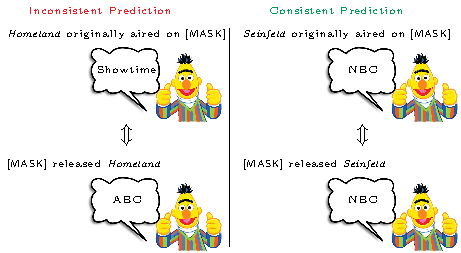
\includegraphics[width=1.\columnwidth]{figures/overview}

\caption{Overview of our approach. We begin with KB tuples (\textit{subject}, \textit{object}), of which we fill into a relational \textit{pattern} the: (\textit{subject}, \textit{[MASK]}) tuple,
% \nk{() are off here, also not sure if "populated" pattern is clear. Maybe also mention that the pattern is an relational pattern.}, 
and feed it into a PLM. 
We expect that a consistent model would predict the same answer for every two patterns $pattern_1$, $pattern_2$ which are paraphrases. 
In the example above, the model makes an inconsistent prediction for the ``Homeland originally aired on [MASK]'' and ``Homeland premiered on [MASK]'' patterns and a consistent prediction on the same two patterns when the subject is `Seinfeld'.
\am{Unclear, and too long. maybe also annotate left side as (a) and right side as (b)}}
\label{fig:overview}
% \vspace{-6mm}
\end{figure}


The recent rise of PLMs sparked a discussion around whether these models can be used as KBs \am{undefined acronym} \cite{lama,petroni2020how,alpaqa,roberts2020much}. 
% \nk{I would also cite this one maybe: "How Much Knowledge Can You Pack Into the Parameters of a Language Model?"}. 
Consistency is a very important property of KBs, and is particularly important in automatically constructed ones.
%However, an important property of KBs, especially in automatically constructed KBs, is consistency.
One of the biggest appeals of using a PLM as a KB \am{comma} is the ability to query it in natural language, instead of relying on a specific schema.
The expectation is that the PLMs \am{remove "the"} would abstract away the language, and map queries in natural language into a meaningful representation \am{plural, meaningful representations}, such that queries with identical intent but different language \am{"different language" also has other connotations. perhaps "different form"?} would yield the same answer. 
For example, the query ``\textit{Homeland} was released on [MASK]'' should produce the same answer as ``\textit{Homeland} was originally aired on [MASK]''. \am{good point to refer to Figure 1}
Studying inconsistencies of PLM-KBs can also teach us about the organization of `knowledge' in the model, or lack thereof. 
Failure to behave in a consistent manner may also point to other issues in representations, 
% \nk{other issues seems a bit vague. Which other ones beside antonyms and synonyms do you have in mind?},
such as the similarity between antonyms and synonyms \cite{nguyen2016integrating}, symmetricity of the representation and the capability to handle negation. \nk{there was a paper studying this in PLMs right. Shouldn't we cite that one here}

In this work, we study consistency from the factual knowledge perspective: we focus on the ability to extract factual information while staying\am{being} invariant to paraphrases.
Our setup relies on zero-shot evaluation, which allows us to inspect these capabilities in models directly, without adding biases that arise from finetuning on a specific dataset \am{plural, specific datasets}. This allows us to assess the extent by which consistency was acquired during pretraining, and to compare models in relation to this property\am{period} %\sr{what does ``progress" mean here?}. %\sr{Question: how do we separate between lack of consistency due to the extraction method (maybe other extraction method would yield more consistent predictions), and an inherent lack of consistency in the model's behavior?}


We introduce a new benchmark that measures consistency in PLMs, using factual knowledge that was found to be partially encoded in them (\S \ref{sec:probe}).
This benchmark, \resource{}, is a manually curated resource
that provides patterns -- short textual prompts -- that are paraphrases of one another, with @@ paraphrases describing 40 binary relations such as \textit{X born-in Y}, \textit{X works-for Y} (\S \ref{sec:rel-graph}).
We then test multiple PLMs for consistency over knowledge, 
expecting a consistent model to predict the same answer for all the patterns of the same relation.
An overview of the probe\am{maybe instead of "the probe" say "our approach"} is presented in Figure \ref{fig:overview}.
Using \resource{}, we probe for consistency in four PLM types: BERT, BERT-whole-word-masking, RoBERTa and ALBERT (\S \ref{sec:setup}).
We find that overall, current models perform poorly on the consistency benchmark, although there is a high variance between the different relations (\S \ref{sec:experiments}). 

Finally, we propose a method that improves the consistency capabilities of models, with an additional consistency loss (\S \ref{sec:adding_consistency}). Models trained with this loss show promising results and achieve better consistency performance on new relations, although there still remains a big gap to achieving fully consistent models.
% Extending upon previous work that showed that factual knowledge can be extracted to some degree \cite{lama,alpaqa}, we extend their proposed patterns that were used to extract that information, and manually write paraphrases to the original patterns.


% \resource{} contains 40 relations from the T-REx dataset \cite{trex} provided by LAMA \cite{lama}, such as: \textit{born-in}, \textit{is-a-citizen}, \textit{works-for}, etc (\S \ref{sec:rel-graph}).
% The paraphrases were built by experts, and provide a high-quality resource.
% \nk{jump from one graph to multiple graphs} 
% Each of these graphs contains between @@-@@ different nodes, where each node is a pattern, e.g. ``[X] was aired on [Y]'', where \textit{[X]} and \textit{[Y]} are slot fillers for a subject and object.
% Moreover, each edge is also annotated with the modification type (e.g. syntactic, lexical) \sr{I am not sure we need to mention these in the intro, given the pretty narrow / heuristic way we define those}.
% Examples of edges of the graphs are displayed in Figure \ref{fig:graph}.


%%%%%%%%%%%%%%%


% By combining the \resource{} with the proposed framework, we are able to test different PLMs and how strong their consistency capabilities are.
